\documentclass[UKenglish,a4paper, 11pt]{article}
\usepackage{amsmath,amssymb}
\usepackage[dvipsnames]{xcolor}
\usepackage{listings}
\usepackage{graphicx}
\usepackage{cleveref}
\author{Nicklas Guldberg}
\title{\LaTeX exercise}
\newcommand{\ex}{\mathrm{ex}}
\lstdefinestyle{sharpc}{language=[Sharp]C, basicstyle=\small, frame=single, backgroundcolor=\color{yellow} }

\lstset{style=sharpc}
\begin{document}

\maketitle
In this exercise we are given the code snippet:
\begin{lstlisting}[breaklines]
static double ex(double x){
if(x<0)return 1/ex(-x);
if(x>1.0/8)return Pow(ex(x/2),2); // explain this
return 1+x*(1+x/2*(1+x/3*(1+x/4*(1+x/5*(1+x/6*(1+x/7*(1+x/8*(1+x/9*(1+x/10)))))))));
}
\end{lstlisting}
The formal definition of the exponential functions is
\begin{equation}
	\exp x = \sum_{k=0}^\infty \frac{x^k}{k!} = 1 + x + \frac{x^2}{2} + \frac{x^3}{6} + \dots
\end{equation}
The factorial makes the higher order terms diminish rather quickly, and we can in good conscience approximate the power series as the first 11 terms,
\begin{equation}
	\exp (x) \approx \mathrm{ex}(x) := 1 + x + \frac{x^2}{2} + \frac{x^3}{6} + \dots + \frac{x^{10}}{10!}. \label{eq:ex}
\end{equation}
If we factor $x$ out we get
\begin{equation}
	\ex (x) = 1 + x\left(1 + \frac{x}{2} + \frac{x^2}{6} + \dots + \frac{x^{9}}{10!}\right)
\end{equation}
Doing this multiple times gets us
\begin{equation}
	\ex (x) = 1 + x \left(1 + \frac{x}{2} \left(1 + \frac{x}{3}\left(1+ \dots\right)\right)\right).
\end{equation}
\begin{figure}[h]
	\centering
	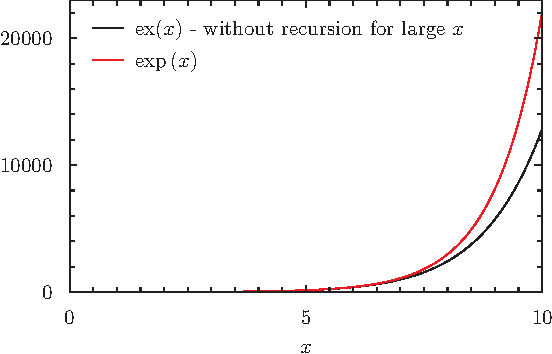
\includegraphics[]{divplot.pdf}
	\caption{$\ex(x)$ diverges from $\exp(x)$ at large $x$. } \label{fig:exdiv}
\end{figure}
Our approximation in \cref{eq:ex} is good for $x$ close to 0, but for higher $x$ it diverges from $\exp (x)$ as can be seen in \cref{fig:exdiv}.	To remedy this we decide to only use the approximation when the argument is $x<1/8$. For $x>1/8$ we can use the property
\begin{align}
	\exp( x) = \exp\left(\frac{x}{2}\right)^2 \approx \ex \left(\frac{x}{2}\right)^2.
\end{align}
Doing this trick multiple times lets us evaluate $\ex (x)$ at any $x$. Finally to avoid writing things twice we use $1/\ex(-x)$ for $x<0$. The method evaluated from $x=-10$ to $x=10$ is plotted in \cref{fig:testplot}.
\begin{figure}[h]
	\centering
	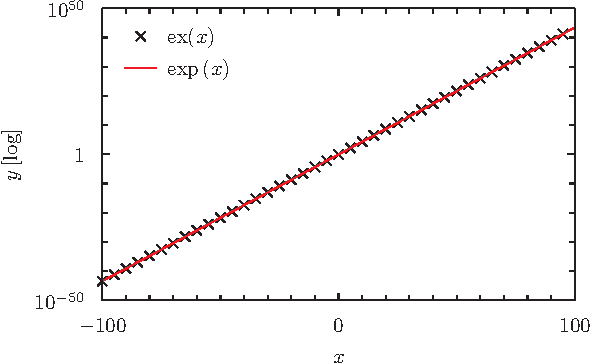
\includegraphics{testplot.pdf}
	\caption{Logarithmic plot of the $\ex (x)$-method against $\exp(x)$.}\label{fig:testplot}
\end{figure}


\end{document}